\section{Вычислительные эксперименты}

В качестве основных датасетов для задачи детекции были выбраны Pascal VOC\cite{pascal-voc-2007} и COCO\cite{DBLP:journals/corr/LinMBHPRDZ14}. Датасет Pascal VOC содержит 20 классов объектов, тогда как COCO включает 80 классов. 

При генерации аугментированного датасета на основе Pascal VOC и COCO мы заменяли объект с наибольшим ограничивающим прямоугольником новым объектом другого класса, выбранным из списка меток Pascal VOC и COCO соответственно. При этом класс исходного объекта заранее удалялся из списка кандидатов, чтобы он не мог быть выбран повторно. Пороговое значение для модели фильтрации составляло 0.23.

Для получения экспериментальных результатов были использованы модели YOLO11n и RTDETR-L из библиотеки Ultralytics. Проведён анализ влияния аугментаций на функцию качества mAP и mAP50:95, а также исследовано влияние отдельных компонентов архитектуры на итоговые значения mAP и mAP50:95. Обучение каждой из моделей детекции выполнялось в течение 500 эпох с нуля, после чего сравнивались максимальные показатели mAP и mAP50:95 на валидационном датасете. Результаты экспериментов приведены в соответствующей таблице 1. 

Ниже представлены примеры объектов из датасетов: на рисунке 1 — исходные изображения, на рисунке 2 — результаты их аугментации, а на рисунке 3 — полученные изображения без отдельных компонентов архитектуры. 

Данные вычислительные эксперименты показывают, что аугментации влияют на разнообразие датасета и улучшают показатель mAP. Кроме того, продемонстрировано, что модель расширения текстового запроса и модель фильтрации являются важными компонентами нашей архитектуры и также влияют на итоговое значение mAP.
% -------------------------------
% Таблица 1: Результаты YOLO
% -------------------------------
% =======================================
%  Таблица 1: YOLO (строки — task_id, столбцы — метрики)
% =======================================




\begin{figure}[htp]
  \centering
 % уменьшает отступ между изображением и подписью

  % первая картинка
  \begin{minipage}[t]{0.4\textwidth}
    \centering
    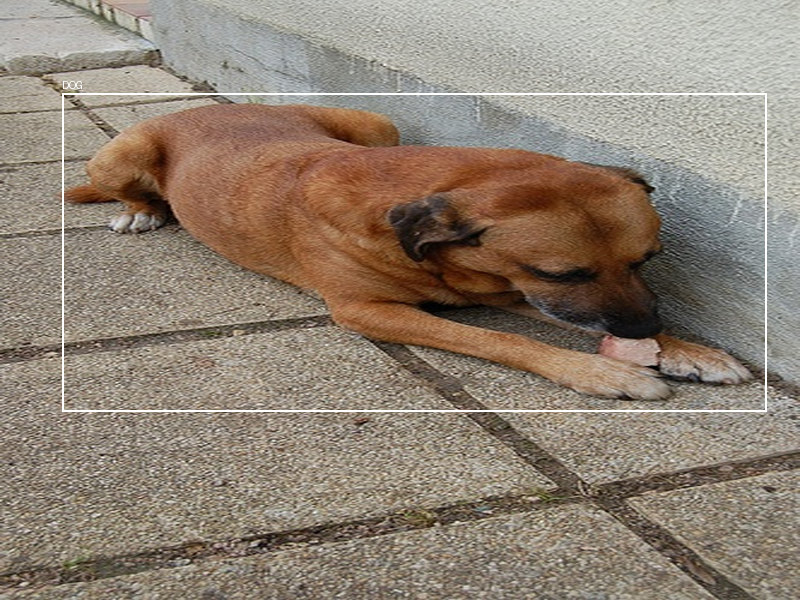
\includegraphics[width=\linewidth]{images/000036.png}
    \label{fig:img1}
  \end{minipage}%
  \hspace{0.05\textwidth}% промежуток между картинками
  % вторая картинка
  \begin{minipage}[t]{0.4\textwidth}
    \centering
    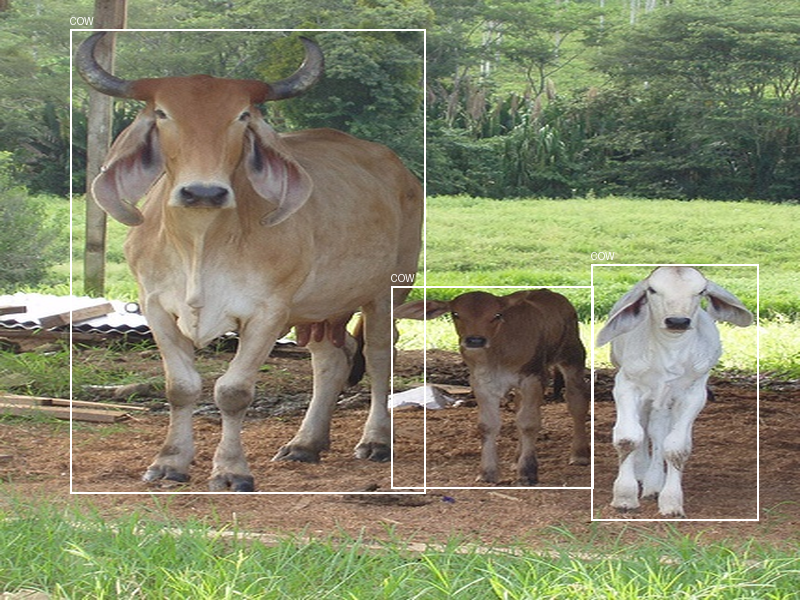
\includegraphics[width=\linewidth]{images/001299.png}
    \label{fig:img1}
  \end{minipage}

  \caption{На левом изображении представлен объект класса «собака»; на правом — объекты класса «корова» из оригинального датасета.}
  \label{fig:comparison}
\end{figure}

\begin{figure}[htp]
  \centering
  % первая картинка
  \begin{minipage}[t]{0.4\textwidth}
    \centering
    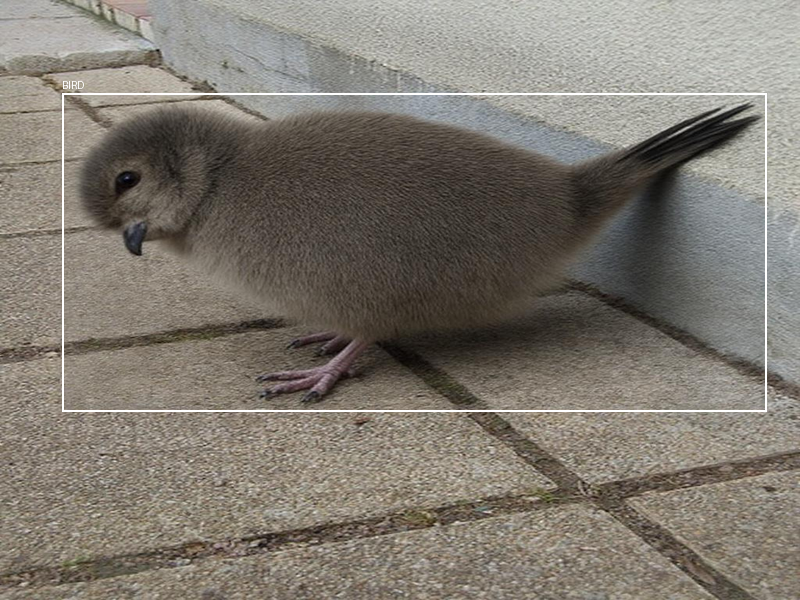
\includegraphics[width=\linewidth]
    {images/aug_000036_with_all.png}
    \label{fig:img2}
  \end{minipage}%
  \hspace{0.05\textwidth}% промежуток между картинками
  % вторая картинка
  \begin{minipage}[t]{0.4\textwidth}
    \centering
    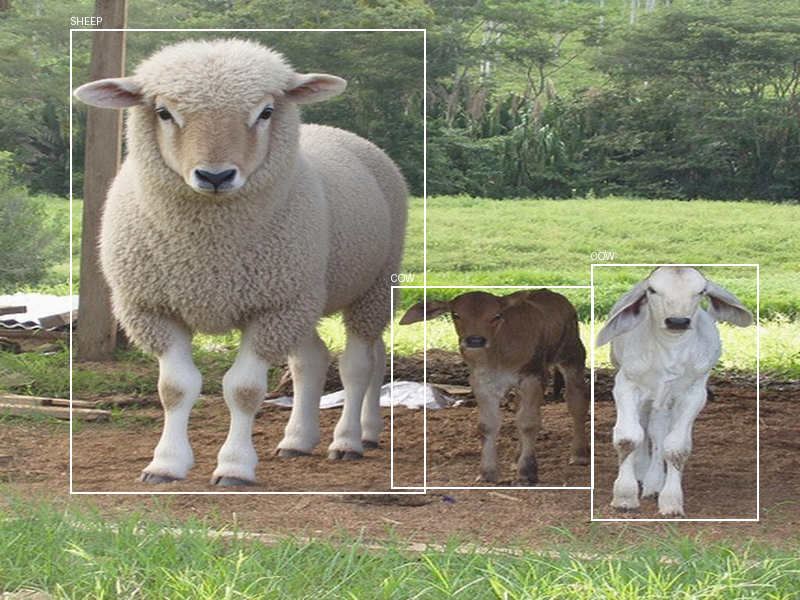
\includegraphics[width=\linewidth]{images/aug_001299.png}
    \label{fig:img2}
  \end{minipage}

  \caption{На левом изображении представлен аугментированный объект класса «птица»; на правом — аугментированный объект класса «овца» и оригинальные объекты класса «корова».}
  \label{fig:comparison}
\end{figure}

\begin{figure}[htp]
  \centering
  % первая картинка
  \begin{minipage}[t]{0.4\textwidth}
    \centering
    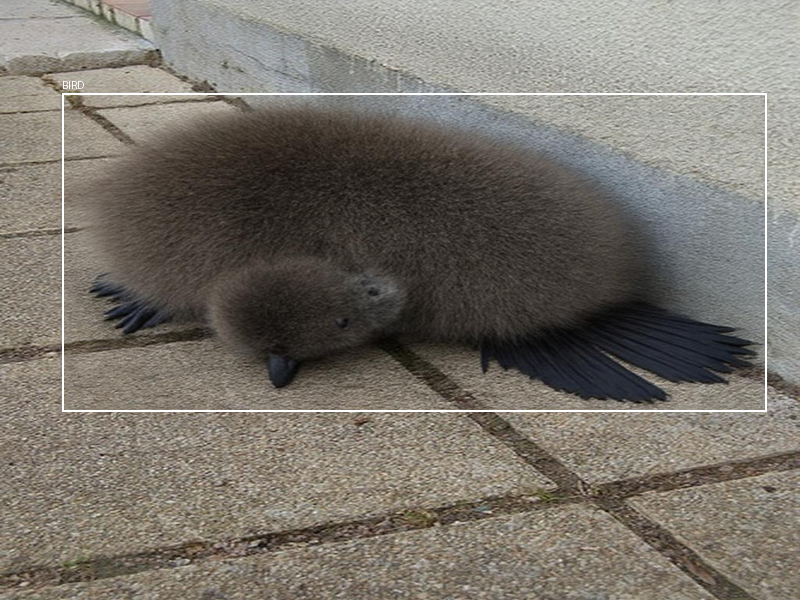
\includegraphics[width=\linewidth]
    {aug_000036.png}
    \label{fig:img3}
  \end{minipage}%
  \hspace{0.05\textwidth}% промежуток между картинками
  % вторая картинка
  \begin{minipage}[t]{0.4\textwidth}
    \centering
    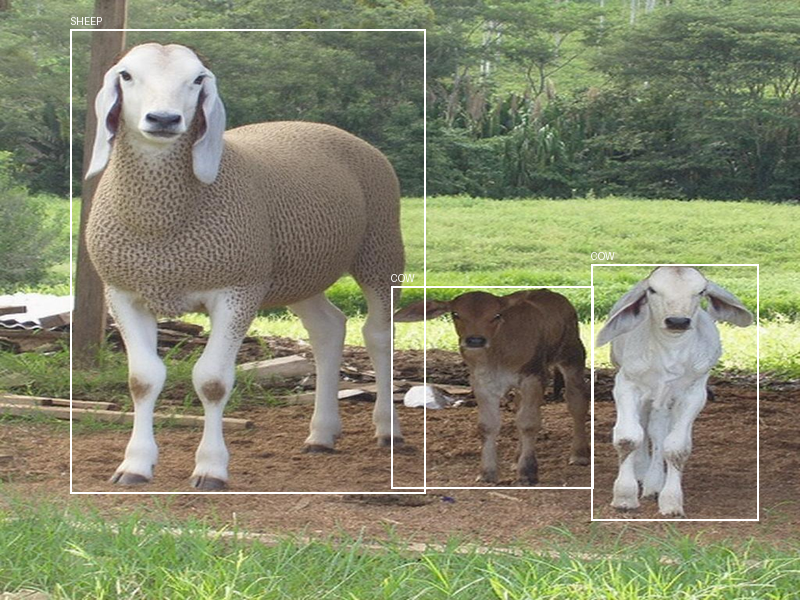
\includegraphics[width=\linewidth]{images/aug_001299_wo_prompt.png}
    \label{fig:img3}
  \end{minipage}

  \caption{На левом изображении представлен аугментированный объект класса «птица», созданный моделью без учёта компонента фильтрации; на правом — аугментированный объект класса «овца» вместе с оригинальными объектами класса «корова», сгенерированный без расширенной подсказки.}
  \label{fig:comparison}
\end{figure}

\vspace{-20pt}

\begin{table}[p]
\centering
\setlength{\tabcolsep}{2.5pt} % Минимальные пробелы
\begin{tabular}{cccc|cc}
\toprule
\textbf{Dataset} & \textbf{Model} & \textbf{Setting} & \textbf{Size} & \textbf{mAP@50} & \textbf{mAP@50:95} \\
\midrule
\multirow{8}{*}{Pascal VOC} 
    & \multirow{4}{*}{DETR}
        & original                     & 4000  & 57.2 & 41.2 \\
        &                              & w/o expanded prompt          & 4000 + 4000  & 55.4 & 38.7 \\
        &                              & w/o filter model             & 4000 + 4000  & 57.4 & 40.9 \\
        &                              & ours                          & 4000 + 4000  & \textbf{58.2} & \textbf{41.4} \\
    \cline{2-6}
    & \multirow{4}{*}{YOLO}
        & original                     & 4000  & 59.6 & 41.5 \\
        &                              & w/o expanded prompt          & 4000 + 4000  & 59.4 & 41.2 \\
        &                              & w/o filter model             & 4000 + 4000  & 61.4 & \textbf{43.2} \\
        &                              & ours                          & 4000 + 4000  & \textbf{61.5} & \textbf{43.2} \\
\midrule
\multirow{8}{*}{COCO} 
    & \multirow{4}{*}{DETR}
        & original                     & 5000 & 26.6 & 17.6 \\
        &                              & w/o expanded prompt          & 5000 + 5000 & 27.5 & \textbf{17.8} \\
        &                              & w/o filter model             & 5000 + 5000 & 26 & 16.5 \\
        &                              & ours                          & 5000 + 5000 & \textbf{27.8} & \textbf{17.8} \\
    \cline{2-6}
    & \multirow{4}{*}{YOLO}
        & original                     & 5000 & 26.7 & 17.4 \\
        &                              & w/o expanded prompt          & 5000 + 5000 & 27.5 & 17.9 \\
        &                              & w/o filter model             & 5000 + 5000 & 27.7 & 17.9 \\
        &                              & ours                          & 5000 + 5000 & \textbf{28.2} & \textbf{18.3} \\
\bottomrule
\end{tabular}
\caption{Сравнение моделей DETR и YOLO, обученных на данных с аугментациями и без, а также анализ влияния отдельных компонентов на значение функций качества mAP.}
\label{tab:augmented-metrics}
\end{table}


% =======================================
%  Таблица: COCO (строки — filename, столбцы — метрики)
% =======================================



% -------------------------------
% Таблица 2: Результаты DETR
% -------------------------------
% =======================================
%  Таблица 1: YOLO (метрики по "наборам данных")
% ======================================


